\section{Auswertung}
\label{sec:Auswertung}
Die LAmorfrequenz der Protonen wird als \SI{21.71134}{\mega\hertz} bestimmt und die ideale Phase ergibt sich als \SI{115}{\degree}.
Eine maximale Amplitude der FID wurde bei $t =  \SI{2.76}{\micro\second}$ gemessen und bei $t = \SI{5.14}{\micro\second}$ verschwindet besagte Amplitude.
Diese Zeiten geben daher die Pulslängen für einen \SI{90}{\degree} und einen \SI{180}{\degree} Impuls.
Die Temperatur der Spule zum Zeitpunkt der Messung wird als \SI{21.1}{\celsius} bestimmt.

\subsection{Bestimmung der $T_1$-Relaxationszeit}
\begin{figure}
    \center
    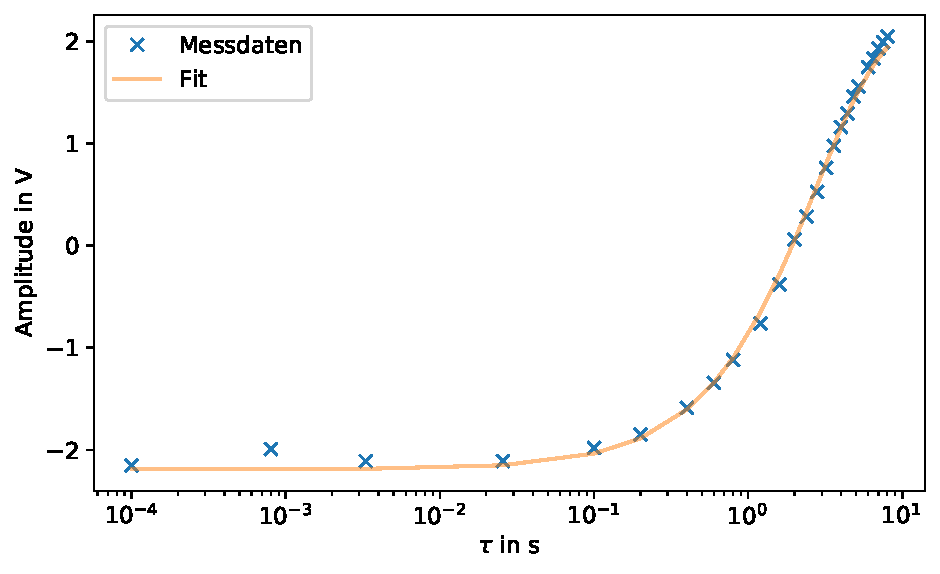
\includegraphics[scale = 1]{plots/df1.pdf}
    \caption{df1}
    \label{fig:df1}
\end{figure}
\begin{align*}
    A_0 &= \SI{2.1912 +- 0.0226}{\volt}\\
    T_1 &= \SI{2.784 +- 0.04}{\second}
\end{align*}
\subsection{Bestimmung der $T_2$-Relaxationszeit}
\begin{figure}
    \center
    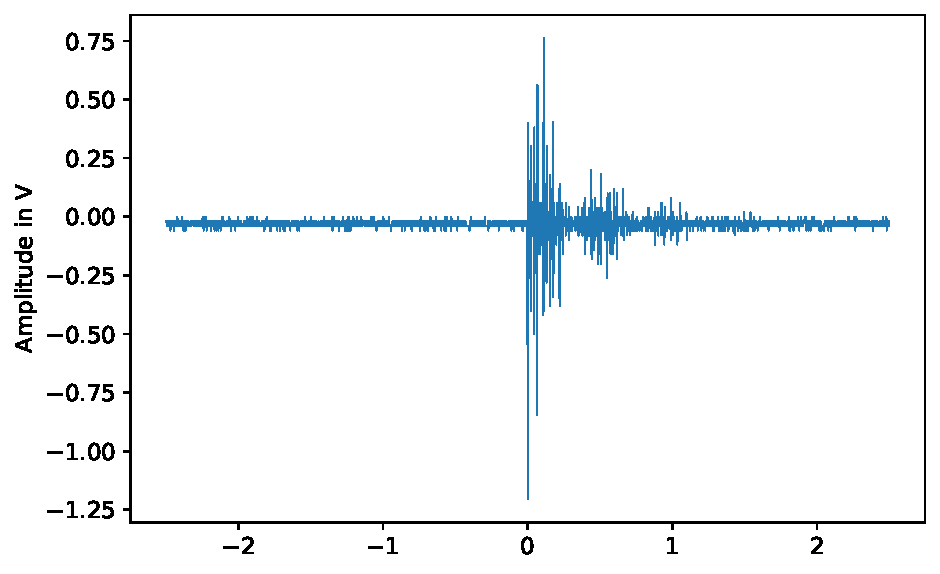
\includegraphics[scale = 1]{plots/df54.pdf}
    \caption{df54}
    \label{fig:df54}
\end{figure}
\begin{figure}
    \center
    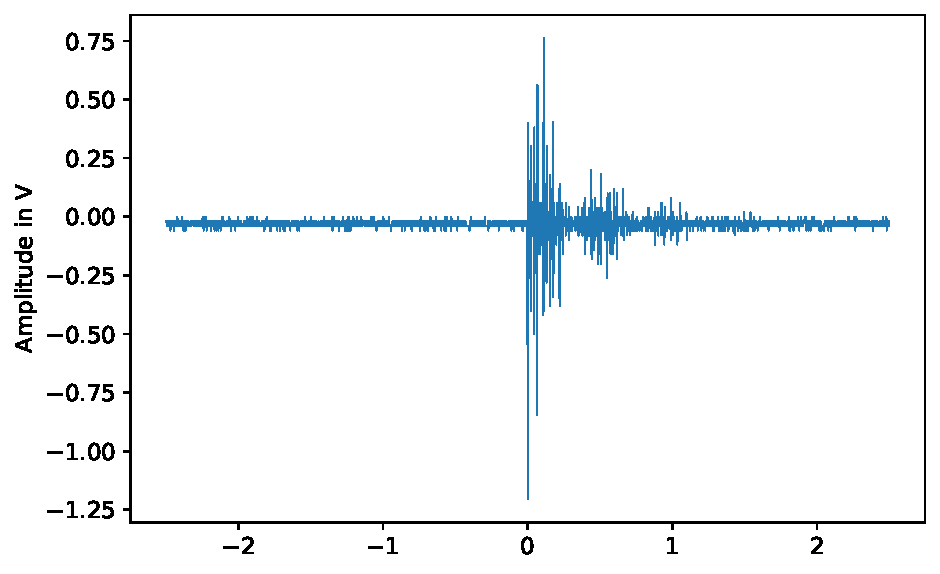
\includegraphics[scale = 1]{plots/df54.pdf}
    \caption{df54}
    \label{fig:df54}
\end{figure}
\begin{align*}
    A_0 &= \SI{0.319 +- 0.009}{\volt}\\
    T_2 &= \SI{0.95 +- 0.08}{\second}
\end{align*}

\subsection{Bestimmung der $T_D$-Relaxationszeit}

\begin{figure}
    \center
    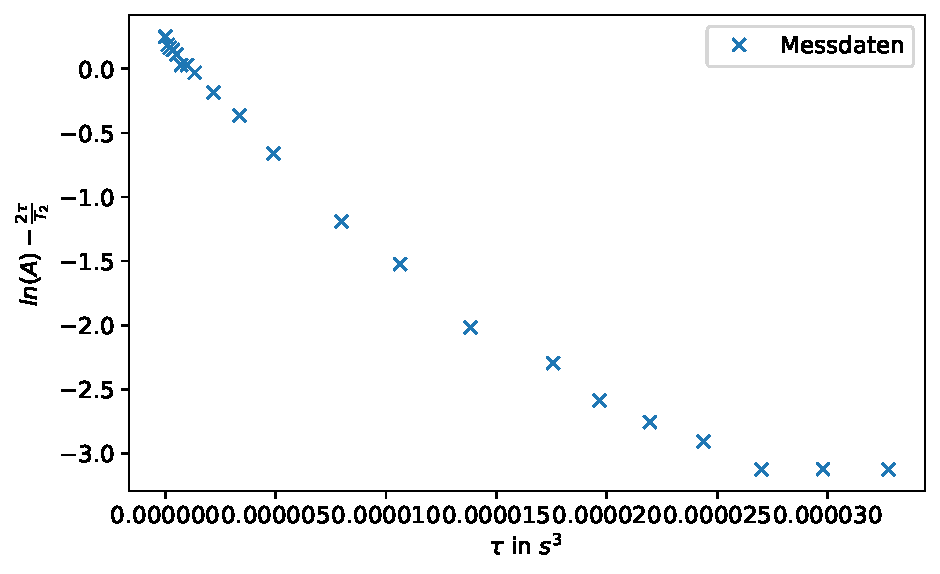
\includegraphics[scale = 1]{plots/df2.pdf}
    \caption{df2}
    \label{fig:df2}
\end{figure}
\begin{figure}
    \center
    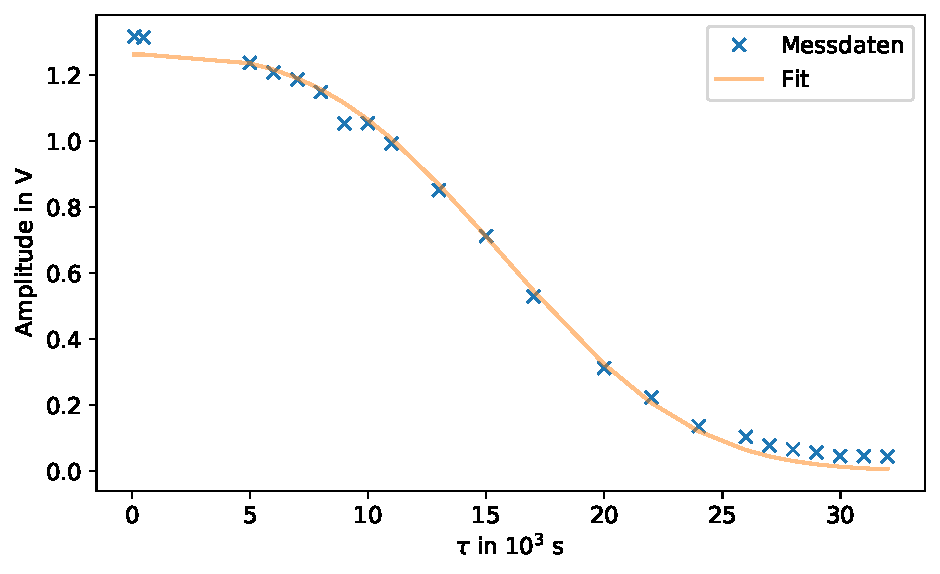
\includegraphics[scale = 1]{plots/df2_2.pdf}
    \caption{df2\_2}
    \label{fig:df2_2}
\end{figure}

\begin{align*}
    A_0 &= \SI{1.2897 +- 0.0127}{\volt}\\
    T_2 &= \SI{5.876 +- 0.207}{\second}
\end{align*}

\begin{figure}
    \center
    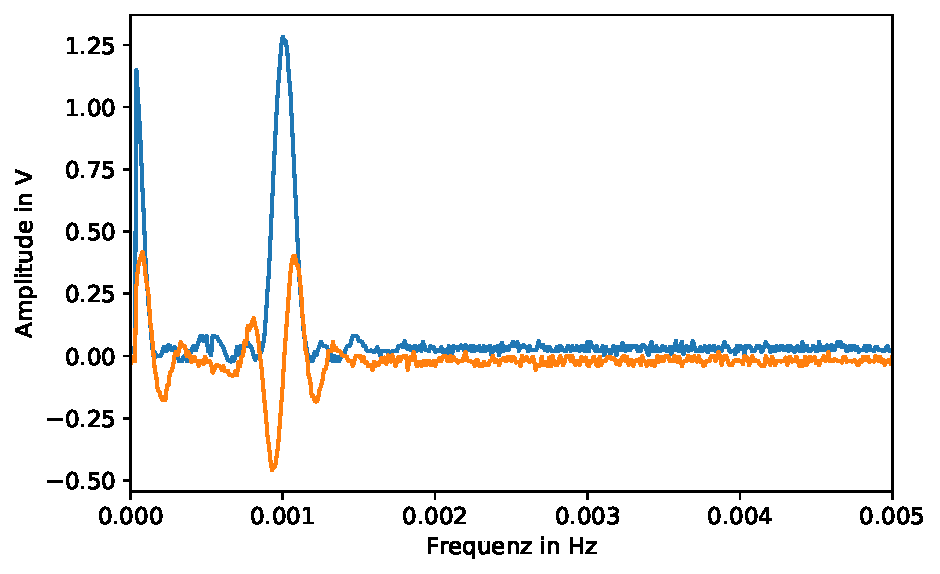
\includegraphics[scale = 1]{plots/df58_59.pdf}
    \caption{df58\_59}
    \label{fig:df58_59}
\end{figure}

\begin{figure}
    \center
    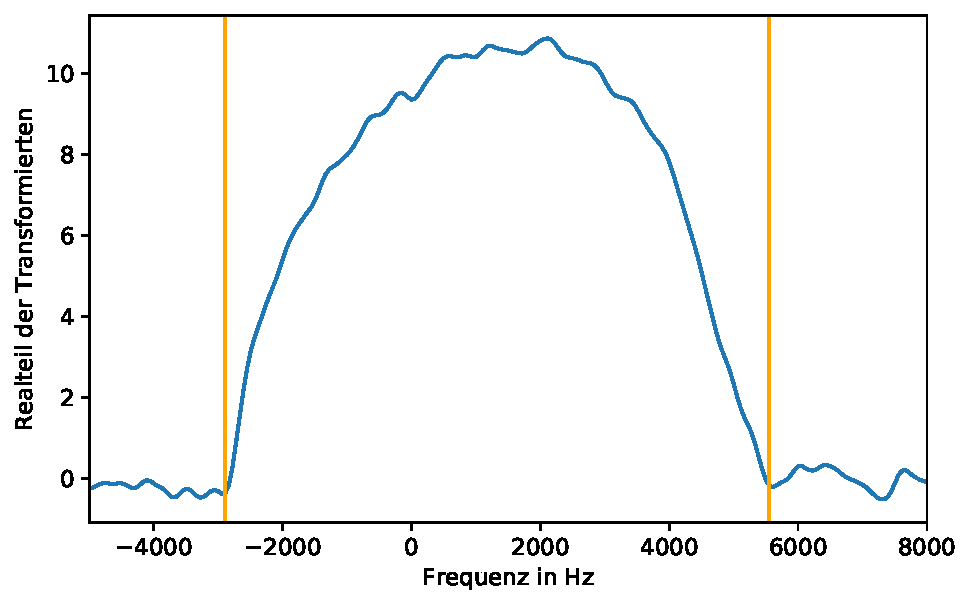
\includegraphics[scale = 1]{plots/fourier.pdf}
    \caption{fourier}
    \label{fig:fourier}
\end{figure}